%=============================================================================
\chapter{Challenges and Applications of Path Planning in Swarm Robots}\label{chap:challenges}
%=============================================================================

This chapter examines the complexities of deploying swarm robots, particularly
with respect to their navigation and coordination, and then reviews the main
domains in which swarms are being applied.

%-----------------------------------------------------------------------------
\section{Challenges in Dynamic and Complex Environments}\label{sec:dynamic-challenges}

With complex obstacles, large search spaces, and unpredictable changes, the
difficulty of path planning increases dramatically. In multi-robot systems,
simultaneous operation creates a risk of collisions between the robots and with
obstacles, which can lead to equipment damage, delays, or mission failure;
collision avoidance therefore becomes a critical challenge
\cite{oh2025survey,lin2022review}.

\subsection{Obstacle Avoidance and Collision Resolution}

In the swarm robotics community, obstacle avoidance is regarded as a basic and
important task. It refers to the ability of robots to move around obstacles
without colliding with them, mimicking the maneuverability observed in
biological swarms \cite{tan2016handbook}.

\subsubsection{Collision Avoidance Strategies in Dynamic Environments}

In a dynamic environment, the ability of the planning algorithm to adjust the
path in real time to accommodate moving obstacles, changes in the layout of the
environment, or relocated targets is essential. The challenge intensifies when
the moving obstacles have unknown headings, which makes accurate prediction of
potential blocking points difficult \cite{li2021rrt}.

The strategies used for collision avoidance in dynamic multi-robot systems
typically emphasize real-time adaptability and computational efficiency:
\begin{itemize}
  \item \lead{Decentralization} The strategies are generally distributed and
        based on local information and communication constraints, which
        contributes to robustness and adaptability \cite{oh2025survey}.
  \item \lead{Real-time replanning} The rapidly-exploring random tree (RRT)
        algorithm and its variants have been adapted to operate in real time in
        dynamic environments. One strategy grafts new waypoints onto the
        existing path based on local obstacle avoidance; by avoiding the
        recomputation of the entire original path when an obstacle is detected,
        it greatly reduces the computation time and reaches the corrected path
        with a relatively short deviation from the initial one \cite{li2021rrt}.
  \item \lead{Learning-based methods} Deep reinforcement learning (DRL) methods
        are increasingly preferred over classical methods because they handle
        collision avoidance in high-dimensional spaces without requiring the
        robots' kinematics or a global map \cite{zhang2025deep,huttenrauch2019deep}.
\end{itemize}

\subsubsection{Potential Force Methods for Collision Avoidance}

The artificial potential field, introduced by Khatib in 1986, is the classical
basis of real-time collision avoidance: the goal attracts, the obstacles repel,
and the robot moves under the resulting force \cite{khatib1986real}.
\begin{itemize}
  \item \lead{Avoidance mechanism} Repulsion from an obstacle has been likened to
        the mechanism of an atomic nucleus: the obstacle generates a virtual
        repulsive force, and the robots maneuver around it like electrons
        \cite{tan2016handbook}.
  \item \lead{Priority and guarantee} The collision avoidance mechanism must take
        precedence over all other actions \cite{sahin2007swarm}. With properly
        defined potential functions, a mathematical guarantee can be given that
        no collision will occur, provided that the repulsive force becomes
        unbounded as the distance tends to zero \cite{khatib1986real}.
  \item \lead{Swarm coordination} Potential functions are used to guide swarms
        and to modify the desired positions of the robots so that they circumvent
        obstacles; shape controllers combine several potential forces to reach a
        formation while avoiding collisions \cite{tan2016handbook}.
\end{itemize}

\subsubsection{Obstacle Enlargement and Robot Shrinking}

A simplifying deterministic technique in path planning is to adjust the effective
size of the obstacles or of the robot in order to simplify collision checking
\cite{lin2022review}.
\begin{itemize}
  \item \lead{Principle} This mechanism achieves collision avoidance by
        effectively enlarging the obstacles and shrinking the moving body to a
        point mass.
  \item \lead{Application} In constrained optimization formulations (such as
        global path planning in a static environment), the radii of convex
        polygonal and circular obstacles are increased in proportion to the
        physical dimensions of the robot. The robot is thus modeled as a
        particle that remains collision-free as long as it stays outside the
        boundary of the enlarged obstacle \cite{tan2016handbook}.
\end{itemize}

\subsubsection{Optimal Reciprocal Collision Avoidance (ORCA)}

ORCA is a powerful and widely used variant of the reciprocal velocity obstacle
(RVO) methods for collision-free navigation \cite{vandenberg2011reciprocal}.
\begin{itemize}
  \item \lead{Mechanism} Assuming that the velocities of the neighbors are known
        and exchanged, ORCA selects a collision-free velocity for each agent in
        real time by solving a small linear program over half-plane constraints.
  \item \lead{Efficiency} For an agent with $k$ neighbors, ORCA takes $O(k)$ time
        \cite{zhou2017fast}.
  \item \lead{Comparison with Voronoi-based methods} ORCA is often compared with
        the buffered Voronoi cell (BVC) method, which has the same complexity and
        similar empirical performance. The key difference lies in the exchange of
        information: ORCA relies on communication to share positions and
        velocities, whereas BVC needs only the sensed relative positions to
        guarantee avoidance \cite{zhou2017fast}.
\end{itemize}

\subsection{Unknown and Dynamic Environments}

The transition from controlled laboratory settings to real-world applications
requires handling environments whose information is incomplete or that change
continuously. Under these conditions, swarm path planning must address real-time
search, robust coordination, and dynamic target seeking.

\subsubsection{Search-and-Rescue Missions in Hazardous Conditions}

Search-and-rescue (SaR) operations are a key target for swarm robotics, because
these scenarios are inherently complex and hostile and challenge the application
of traditional multi-robot systems \cite{tan2016handbook}.
\begin{itemize}
  \item \lead{Characteristics of SaR environments} Large extents, from hundreds
        of square meters to hectares; strong dynamics caused by the agents
        themselves and by external events such as collapses, fires, floods, and
        earthquakes; and harsh conditions, including abrasive dust, water,
        chemicals, and numerous obstacles that damage the hardware and disrupt
        communication \cite{tan2016handbook}.
  \item \lead{Advantages of swarms} Robustness to the failure of units,
        scalability, and reliance on self-organization improve the emergency
        response through damage assessment, resource management, and movement
        through complex environments to find and assist survivors. Examples
        include aquatic drones searching flooded areas and nano-robots proposed
        for cleaning up hazardous materials \cite{bhowmick2024bio}.
\end{itemize}

\subsubsection{Adapting to Moving Targets and Changing Conditions}

An important challenge arises when the targets, the obstacles, or the terrain are
not fixed but change dynamically and unpredictably \cite{tan2016handbook,lin2022review}.
\begin{itemize}
  \item \lead{Handling dynamic changes} Swarm systems must react and adapt in real
        time to changes in the terrain, in environmental conditions (such as
        weather and currents), or to unexpected obstacles, for example shifting
        debris after a disaster \cite{bhowmick2024bio}.
  \item \lead{Moving target tracking (MTT)} In an environment full of obstacles,
        the swarm must simultaneously move as a flock, avoid the obstacles, and
        maintain enough collective coverage that a randomly moving target never
        leaves its sight; this problem is relevant to escorting, monitoring, and
        group transport \cite{tan2016handbook}.
  \item \lead{Difficulty of prediction} In environments with moving obstacles
        whose headings are unknown, determining the potential blocking points is
        difficult \cite{li2021rrt}.
  \item \lead{Adaptive algorithms} Continuous motion and adaptation call for
        algorithms with predictive capabilities, such as bio-inspired optimizers
        that model warning behavior for cooperative planning in dynamic
        environments \cite{lin2022review}.
\end{itemize}

\subsubsection{Real-Time Path Planning for Multi-Robot Systems}

In dynamic, unknown, or partially known environments, computing an optimal global
path is often prohibitively expensive, so the focus shifts to efficient real-time
local strategies for planning and replanning:
\begin{itemize}
  \item \lead{Dynamic grid search (\Dstar{} and \Dstar{} Lite)} \Dstar{} extends
        \Astar{} to changing maps: by updating the weights of the edges affected
        by newly observed obstacles, it repairs only the necessary parts of the
        path instead of replanning completely \cite{stentz1994optimal,koenig2002d}.
  \item \lead{Time rolling windows} Combined with local optimizers such as ABC,
        PSO, or the fireworks algorithm, a rolling time window in which each
        robot perceives and predicts its surroundings replaces costly global
        planning in dynamic and unknown environments \cite{tan2016handbook}.
  \item \lead{RRT-based real-time replanning} The RRT family is well suited to
        dynamic environments because it accounts for the dynamic constraints of
        the robot; grafting adds new waypoints to the existing path, which
        reduces the computational load of a complete recomputation
        \cite{li2021rrt}.
  \item \lead{Artificial potential field} The APF is valuable for rapid path
        adjustment because of its fast reaction to nearby obstacles, but it is of
        limited use in highly complex environments because of the risk of getting
        trapped in local minima (\cref{fig:apf}) \cite{zhang2023multi}.
\end{itemize}

\subsection{Adaptation and Real-Time Replanning}

The growing demand for deploying multi-robot systems in complex real-world
scenarios has made it necessary to move from offline, static planning to
strategies for real-time adaptation and rapid replanning.

\subsubsection{Dynamic Multi-Robot Systems and Environmental Changes}

Path planning in dynamic environments is multifaceted: the environment changes
because of external factors, moving targets, or the actions of the robots
themselves \cite{tan2016handbook}.
\begin{itemize}
  \item \lead{Need for real-time reaction} Algorithms must adapt quickly to
        changes; traditional deterministic methods often fail to adapt rapidly to
        unexpected obstacles and are computationally expensive \cite{abujabal2024path}.
  \item \lead{Environmental instability} In applications such as SaR after
        natural disasters, the environment can change rapidly (falling debris,
        weather conditions, unexpected events), and the algorithms must allow the
        behavior and the flight or motion patterns to be changed immediately
        \cite{bhowmick2024bio}.
  \item \lead{Adaptability and flexibility} The swarm must be flexible enough to
        cope with various tasks and situations and to adjust its paths as water
        or air currents change or as obstacles appear \cite{tan2013research}.
  \item \lead{Complexity of distributed control} Controlling groups of simple,
        reactive robots in a distributed structure is difficult, because the
        desired macroscopic behaviors emerge only from local interactions, and
        path planning must respond to continuously changing scenarios without
        relying on a limited set of predefined conditions
        \cite{brambilla2013swarm}.
\end{itemize}
This demand for adaptability has pushed research toward learning-based methods,
which let robots improve their strategies from experience
\cite{kuckling2023recent}.

\subsubsection{RRT-Based Algorithms for Replanning}

The RRT family and its variants are suitable for dynamic environments because of
their ability to generate feasible paths and to incorporate the dynamic
constraints of the robot directly \cite{li2021rrt}.
\begin{itemize}
  \item \lead{RRT-Connect and optimality} RRT and its enhanced versions, such as
        RRT-Connect and \RRTstar, have been explored in dynamic environments;
        although \RRTstar{} provides asymptotic optimality, it can be
        computationally expensive \cite{chen2025survey}.
  \item \lead{Grafting for real-time efficiency} Grafting adds new points based on
        local avoidance and nonholonomic constraints, generating a new point when
        a potential collision is detected in the next sampling step. Instead of
        recomputing the whole tree, only a short detour results \cite{li2021rrt}.
\end{itemize}

Dynamic variants include \cite{chen2025survey}:
\begin{itemize}
  \item \lead{DRRT} Provides fast, feasible, but sub-optimal paths by pruning and
        regrowing the affected parts of the tree.
  \item \lead{\RRTstar FND} Achieves asymptotic optimality through repeated
        updates in a dynamic environment, albeit at a high computational cost.
  \item \lead{RT-\RRTstar} Retains the full tree structure without pruning, which
        enables fast queries for multiple goals and rapid rewiring of the path in
        response to dynamic obstacles and changing goals.
\end{itemize}

%-----------------------------------------------------------------------------
\section{Scalability and Robustness}\label{sec:scalability}

Scalability and robustness are common and essential properties of swarm systems
that enable them to operate effectively in complex real-world scenarios.
Robustness refers to the ability of the system to function normally despite
disturbances or individual failures, whereas scalability refers to the ability
to maintain effective operation across different population sizes
\cite{dias2021swarm,brambilla2013swarm}.

\subsection{Scalability in Swarm Systems}

Scalability is both a critical challenge and a defining characteristic of swarm
robotics: the system must work with arbitrary population sizes, from a few units
to potentially thousands. Since the control method is usually identical for every
member of the swarm, the system is designed to be highly scalable
\cite{dias2021swarm,tan2013research}.

\subsubsection{Maintaining Performance as the Number of Robots Increases}

Scalability is the capacity of the system to adjust the number of robots flexibly
without a noticeable change in its overall functionality or an excessive drop in
efficiency or reliability \cite{dias2021swarm,tan2013research}.
\begin{itemize}
  \item \lead{Design principle} Scalability stems from decentralization and from
        predominantly local interactions. Methods that rely on global
        broadcasting or on monitoring large parts of the swarm are avoided in
        order to preserve scalability, and local sensing and communication
        facilitate this property \cite{brambilla2013swarm}.
  \item \lead{Ideal versus actual performance} In the ideal case, a
        super-scalable system performs almost independently of the number of
        robots; in a merely scalable system, the loss of efficiency as units are
        added is small; in an unscalable one, population growth causes severe
        degradation or failure \cite{tan2013research}.
  \item \lead{Cognitive complexity} For independently operated robots, the
        operator's workload grows as $O(n)$, whereas with proper distributed
        coordination, swarm control can bring it down to $O(1)$
        \cite{hart2004reducing,kolling2016human}.
  \item \lead{Effect on tasks} Adding or removing members should not jeopardize
        the completion of the mission, and implicit reallocation of tasks should
        occur without external intervention \cite{tan2013research}.
  \item \lead{Challenges} As the number of robots increases, maintaining
        productivity becomes harder and requires mechanisms such as control
        hierarchies and clustering to manage the communication and processing
        load and to prevent bottlenecks \cite{bhowmick2024bio}.
\end{itemize}

\subsubsection{Simulation of Large-Scale Swarms}

Because swarm algorithms are meant to scale to populations that are hard to
build physically, simulating hundreds or thousands of robots is a vital part of
research, and modeling and simulation are the necessary tools for this purpose
\cite{dias2021swarm,hamann2018swarm}. Notable simulators and platforms include:
\begin{itemize}
  \item \lead{ARGoS} A modular simulator that can run several physics engines in
        parallel; it can simulate 10,000 e-pucks in 60\% of the time the real
        experiment would take \cite{dias2021swarm,pinciroli2012argos}.
  \item \lead{Player/Stage/Gazebo} An open-source framework with multi-robot
        capabilities; for 2-D swarm behaviors, its run time scales approximately
        linearly up to at least 100,000 simple robots \cite{tan2016handbook}.
  \item \lead{Kilobot} A low-cost, small physical platform built to test collective
        algorithms with hundreds to thousands of robots; a thousand Kilobots have
        self-assembled into programmed shapes \cite{rubenstein2014programmable}.
\end{itemize}

\subsubsection{Exponential Growth of States in Modular Robotics}

Although scalability usually refers to functioning independently of the size of
the population, in modular robotic systems the complexity of a configuration
space with many degrees of freedom poses a distinct challenge \cite{yim2007modular}.
\begin{itemize}
  \item \lead{Modular systems} Self-reconfigurable systems such as M-TRAN, ATRON,
        and PolyBot are designed to build and form complex structures.
  \item \lead{State explosion} The number of possible configurations grows
        exponentially with the number of modules, which makes centralized
        planning and control difficult and reinforces the need for robust local
        rules.
\end{itemize}
If each of $n$ modules can be in one of $k$ states, the number of combinations is
\begin{equation}
  S = k^{n},
  \label{eq:state-explosion}
\end{equation}
before connectivity constraints are taken into account. Chain-type modular robots
are particularly versatile, but managing this explosion remains a key
computational obstacle \cite{yim2007modular}.

\subsection{Robustness and Fault Tolerance}

Robustness and fault tolerance are fundamental properties of swarm robotic
systems; they mean maintaining operation and a desired level of performance in
the face of internal failures or external disturbances
\cite{dias2021swarm,brambilla2013swarm}.

\subsubsection{Robustness to Failures of Individual Robots}

Robustness to individual failures stems mainly from redundancy and from the
absence of a centralized point of control \cite{dias2021swarm,tan2013research}.
\begin{itemize}
  \item \lead{Massive redundancy} The large number of robots provides critical
        redundancy for safety and fault tolerance, and the loss of one robot can
        be compensated for by the others.
  \item \lead{Distributed control} The absence of a single point of failure means
        that the failure of one node or part does not disable the whole system.
  \item \lead{Performance preservation} The design treats individuals as
        dispensable, so a swarm can lose a considerable share of its robots
        before the mission has to be abandoned, albeit with reduced capability
        \cite{tan2016handbook}.
  \item \lead{Fault detection} The natural redundancy of the swarm can be used to
        detect faulty robots; for example, robots that flash in synchrony, like
        fireflies, can flag a peer that falls out of step as faulty
        \cite{brambilla2013swarm}.
\end{itemize}

\subsubsection{Fault Tolerance and Redundancy in Communication}

Ensuring the robustness of communication in dynamic and crowded environments is
challenging and requires special mechanisms to cope with failures, interference,
and delays \cite{bhowmick2024bio}.
\begin{itemize}
  \item \lead{Redundant communication paths} Establishing alternative paths helps
        maintain the robustness of the network if one path is broken.
  \item \lead{Distributed nodes and reconfiguration} Distributing communication
        tasks among several robots and reconfiguring the network dynamically
        adapt it to changing conditions and reduce the impact of faults.
  \item \lead{Information redundancy} Replicating critical information across
        several robots preserves its availability in the face of communication
        problems.
  \item \lead{MANETs and multi-connectivity} In missions such as SaR, the robots
        must maintain a mobile ad hoc network (MANET) without pre-existing
        infrastructure, using attractive forces and redundancy to stay
        connected. The notion of $k$-connectivity generalizes bi-connectivity:
        the network stays connected as long as fewer than $k$ nodes fail, that
        is, when its vertex connectivity satisfies $\kappa(G) \ge k$
        \cite{tan2016handbook}.
\end{itemize}

%-----------------------------------------------------------------------------
\section{Task Allocation and Coordination}\label{sec:task-allocation}

Multi-robot task allocation (MRTA) is the problem of assigning tasks to
individual robots so as to maximize the expected performance of the overall
system, and it is usually treated as an instance of the optimal assignment
problem. In swarm robotics, this coordination is vital for distributing the work
and ensuring that collective goals are achieved efficiently under decentralized
control \cite{brambilla2013swarm,yan2013survey}.

\subsection{Dynamic Task Allocation}

Dynamic task allocation refers to strategies in which the matching between tasks
and robots is computed repeatedly over time, so that the robot team adapts to
changing conditions, tasks, or environments; online allocation can react to such
changes, whereas simple offline methods cannot \cite{yan2013survey}.

\subsubsection{Efficient Achievement of Collective Goals}

Achieving collective goals requires a distribution of tasks that takes into
account the capabilities of the robots, their workload, and the environmental
constraints, so as to maximize the performance of the whole swarm and minimize
unnecessary redundancy \cite{brambilla2013swarm}.
\begin{itemize}
  \item \lead{Task partitioning} Decomposing tasks greatly improves efficiency.
        In sequential tasks, robots can measure how long they wait for another
        subtask to be completed and use this local cue to decide whether to
        partition the work, so that interdependent subtasks run concurrently and
        interference is reduced \cite{brambilla2013swarm}.
  \item \lead{Decentralized decision-making} For scalability and robustness, each
        robot selects and prioritizes tasks based on its own state, its sensor
        data, and the mission goals \cite{bhowmick2024bio}.
  \item \lead{Optimization objectives} Criteria such as minimizing the completion
        time, maximizing resource utilization, or balancing the load among robots
        are used; maximizing collective utility when group dynamics affect
        performance is in general NP-hard \cite{yan2013survey}. Consensus-based
        allocation has been used to make the assignment both fast and
        energy-efficient \cite{mahato2023consensus}.
\end{itemize}

\subsubsection{Heuristic Algorithms for Distributed Task Selection}

The distributed task selection problem in a swarm is NP-complete, so
polynomial-time heuristics are used to obtain good-enough solutions
\cite{sahin2007swarm}.
\begin{itemize}
  \item \lead{Model and objective} The mechanism tries to assign the desired number
        of swarm units to each task while reducing inter-task delays and
        communication overhead.
  \item \lead{Performance of the heuristics} Heuristics in which each unit
        considers both the effect of the other units on the tasks and its own
        relative position give better task processing and a better distribution
        of units over the tasks.
  \item \lead{Communication constraints} These approaches work without a central
        location or shared memory, using only distributed communication.
\end{itemize}
Auction- and market-based methods are the main alternatives to such heuristics
\cite{yan2013survey}.

\subsubsection{Task Scheduling in Layered Architectures}

In hierarchical or layered architectures, a scheduling layer manages the overall
flow of the mission: at each instant, it selects the subset of tasks that should
run concurrently, elects the robot that coordinates them, and decides how many
tasks to request from each deployment point. A global planner may propose the
allocation, which the scheduling layer then distributes to the swarm; the point
is to approximate a good strategy for the robots' navigation controllers at a
small computational cost while respecting the timing and ordering constraints of
the tasks \cite{yan2013survey,liu2019distributed}.

\subsection{Cooperative Control and Manipulation}

Cooperative control is the problem of steering a multi-agent system toward a
common goal (exploration, search, rescue, etc.); integrating multiple robots
increases capacity, flexibility, and efficiency \cite{yan2013survey}.

\subsubsection{Multi-Robot Teamwork Strategies}

For cohesive and efficient operation, multi-robot systems require coordination
strategies that ensure inter-robot communication, effective task allocation, and
conflict resolution \cite{yan2013survey}.
\begin{itemize}
  \item \lead{Decentralized coordination} For scalability and robustness,
        coordination must be decentralized and based on local interactions and
        simple rules, so that global behaviors emerge from local interactions
        \cite{brambilla2013swarm}.
  \item \lead{Implicit versus explicit} Cooperation can emerge implicitly from the
        autonomous decisions of individuals or be supported by explicit
        communication (subject to bandwidth constraints) to improve information
        exchange and motion synchronization.
  \item \lead{Behavioral approaches} Behavior-based formation control and
        distributed control manage interactions and resolve conflicts with local
        information; a controller based on several potential forces can steer
        the robots toward the desired shape and prevent collisions
        \cite{tan2016handbook}.
  \item \lead{Hierarchical architectures} Hybrid-HASP
        (\cref{sec:control-architectures}) combines competitive and cooperative
        mechanisms to select and combine elementary behaviors, and it supports
        cooperation through implicit communication with simple attractive and
        repulsive signals \cite{tan2016handbook}.
\end{itemize}

\subsubsection{Cooperative Grasping and Object Transport}

Cooperative transport and manipulation (e.g., box pushing) is a common benchmark
and usually involves objects that a single robot cannot handle
\cite{bonabeau1999swarm,brambilla2013swarm}.
\begin{itemize}
  \item \lead{Physical requirements} A physical connection (self-assembly) is
        necessary to cross large gaps or to perform complex transport;
        cooperative grasping requires communication and docking before
        execution.
  \item \lead{The Swarm-bot project} This project showed that autonomous agents
        relying solely on local information can cooperatively transport heavy
        objects that a single robot cannot move; the aggregation of s-bots into a
        formation plays a key role \cite{mondada2003swarmbot,gross2006object}.
  \item \lead{Coordinated motion} In cooperative transport, the robots must share
        information about the object and the destination, agree on a common
        direction, and then move together; Hybrid-HASP has been used to
        coordinate box pushing \cite{tan2016handbook}.
\end{itemize}

\subsubsection{Consensus, Tracking, and Containment}

Path planning for cooperative swarms must address the fundamental objectives of
consensus, maintenance of relative positions or formation (tracking), and
containment \cite{li2014cooperative}.
\begin{itemize}
  \item \lead{Consensus control} The group must reach agreement on the variables
        of interest; consensus algorithms, close relatives of distributed linear
        algorithms, typically move each agent toward the average of the values it
        receives \cite{bullo2009distributed}.
  \item \lead{Tracking and formation control} Formation is a key application of
        cooperative control whose aim is to achieve a fixed geometric pattern;
        leader--follower and flocking approaches are used, the latter with
        collision avoidance, velocity matching, and flock centering
        \cite{reynolds1987flocks,li2014cooperative}. A simulation of
        leader--follower tracking is shown in \cref{fig:leader-follower}.
  \item \lead{Containment and region control} In region control, the group is kept
        within a predefined region using constraint functions, and in multilevel
        designs, the robots converge to the region and form the shape level by
        level \cite{tan2016handbook}.
\end{itemize}
With several leaders, containment requires every follower to stay in the convex
hull spanned by the leaders,
\begin{equation}
  x_i(t) \in \operatorname{conv}\bigl\{x_j(t) : j \in \mathcal{L}\bigr\},
  \label{eq:containment}
\end{equation}
where $\mathcal{L}$ is the set of leaders \cite{li2014cooperative}.

\begin{figure}[htbp]
  \centering
  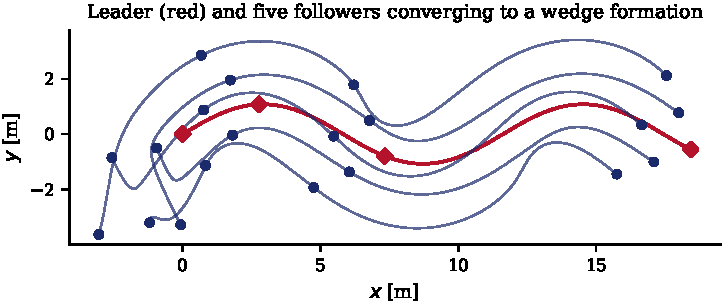
\includegraphics[width=0.85\linewidth]{leader-follower}
  \caption{Leader--follower formation tracking: five followers start from random
           positions and converge, through local consensus on their formation
           errors, to a wedge around the leader (markers every few seconds).}
  \label{fig:leader-follower}
\end{figure}

%-----------------------------------------------------------------------------
\section{Real-World Applications of Swarm Robotics}\label{sec:applications}

The ultimate goal of swarm robotics research is to deploy these systems in
real-world scenarios, especially where the tasks are too hazardous, complex, or
large-scale for individual robots or human teams. Although swarm robotics has
long been confined to academia, the field is moving toward practical
applications \cite{kegeleirs2025towards,shahzad2023review}. Examples are compiled
in \cref{tab:applications} and discussed below.

\begin{table}[htbp]
  \centering
  \caption{Examples of real-world applications of swarm robotics.}
  \label{tab:applications}
  \small
  \rowcolors{2}{lightbg}{white}
  \begin{tabularx}{\linewidth}{@{}>{\bfseries\raggedright\arraybackslash}p{0.18\linewidth}LLL@{}}
    \toprule
    \rowcolor{white}
    Application domain & \textbf{Specific tasks and missions}
      & \textbf{Example platforms or projects} & \textbf{Key advantages and methods} \\
    \midrule
    Agriculture & Precision weeding, crop monitoring
      & LettuceBot, senseFly \cite{bhowmick2024bio}
      & Less herbicide through machine vision; continuous monitoring \\
    Search and rescue & Locating survivors in rubble, flood response
      & RoboBees, AquaDrones \cite{bhowmick2024bio}
      & Rapid area coverage; operation without GPS or infrastructure \\
    Construction & Bricklaying, site inspection
      & Skycatch \cite{bhowmick2024bio}
      & Parallel work and faster construction \\
    Environmental monitoring & Water quality, marine pollution
      & microUSV, CoCoRo \cite{dias2021swarm,shahzad2023review}
      & Distributed sensing and collective mapping \\
    Warehousing and logistics & Goods handling in warehouses
      & Kiva \cite{shahzad2023review}
      & Decentralized path coordination in crowded spaces \\
    Space exploration & Resource prospecting, in-space assembly
      & Swarmies, Marsbees \cite{shahzad2023review}
      & Redundancy and fault tolerance far from help \\
    \bottomrule
  \end{tabularx}
\end{table}

\subsection{Search and Rescue}

\subsubsection{Exploring Hazardous Environments}

Disaster sites are hostile, dynamic, and large, with dust, water, chemicals, and
debris, and these conditions cannot be handled by simply adapting traditional
planning and control \cite{tan2016handbook}. Swarms survive such conditions
through redundancy, and they can map collapsed structures and identify hazards,
locate trapped survivors by body heat, heartbeat, or sound, and track chemical or
radiation leaks \cite{bhowmick2024bio}. Proposed and demonstrated examples
include insect-sized flying robots (RoboBees) for searching collapsed buildings,
aquatic drones (AquaDrones) and amphibious robots for floods, and swarms for
demining \cite{bhowmick2024bio}.

\subsubsection{Initial Deployment and Communication in Faulty Environments}

Two open problems in real SaR missions are the initial deployment of the robots
and the integrity of their network \cite{tan2016handbook}. The initial placement
strongly affects the efficiency of the search; options include random
deployment, contextual deployment that uses map or network-quality information,
and marsupial deployment, in which a larger robot carries and releases smaller
ones. Communication is hard because obstacles are everywhere, the topology of the
MANET keeps changing, and low batteries make nodes fail. Simple range-based rules
are unreliable, so approaches refresh connectivity tables continuously and limit
the robots' motion to keep multi-hop routes of sufficient quality. Virtual
attractive forces based on signal strength keep a robot close to its neighbors
while repulsive forces prevent collisions, and redundancy lets the remaining
robots fill the gap left by one that loses contact \cite{tan2016handbook}.

\subsection{Environmental Monitoring and Mapping}

\subsubsection{Mapping Scalar Fields and Marine Environments}

A common mission is to map an unknown scalar field, such as temperature,
salinity, or pollutant concentration, over a large area, which suits mobile robot
networks. In one cooperative scheme, each robot runs two distributed consensus
filters: a weighted-average consensus filter estimates the field value, an
average consensus filter estimates the confidence of that estimate, and the map
is refined with a weighted-average protocol as the robots move
\cite{tan2016handbook}. At sea, the CoCoRo project used 41 heterogeneous
underwater vehicles, communicating through electric fields and sonar, for
environmental monitoring, while the Platypus system uses swarms of surface
vessels to map water quality and stratify salinity and oxygen levels
\cite{shahzad2023review}.

\subsubsection{Chemical Plume Tracing and Source Localization}

Chemical plume tracing (CPT) steers robots, instead of people, toward the source
of toxic gas leaks, fires, or explosives. It is hard in natural environments
because the source strength and the advection distance are unknown and the plume
is intermittent and meandering under turbulent, time-varying flow. CPT strategies
are often taken from insects, notably moths, using anemotaxis, chemotaxis, and
their combination. In swarm CPT under formation control, a leader performs the
moth-inspired maneuvers and the others keep the formation; robots that can switch
roles outperform a single robot. Since physical experiments are hard to repeat,
simulation platforms based on computational fluid dynamics are essential for
testing these algorithms under identical conditions \cite{tan2016handbook}.

\subsubsection{Area Coverage for Environmental Assessment}

Coverage requires a group of robots to visit every position of an area, usually
discretized into a grid; in dynamic coverage, robots with limited-range sensors
keep moving and sampling until a required coverage level is reached
\cite{muhsen2024survey}. ACO-style virtual pheromones mark explored areas so that
others avoid redundant visits, and PSO-style updates spread the robots over large
areas \cite{nguyen2024swarm}. For photovoltaic parks, a multi-objective ACO
planner adapts the flight paths to wind and moving obstacles and improves both
travel time and coverage (\cref{sec:path-planning-basics})
\cite{ziouzios2025energy}.

\subsection{Agriculture}

Swarm robotics addresses labor shortages and the need for sustainable food
production \cite{bhowmick2024bio,seebacher2025collective}.
\begin{itemize}
  \item \lead{Harvesting and plant care} Swarm systems for autonomous harvesting
        use computer vision and machine learning to pick ripe crops and a
        decentralized architecture for flexibility and robustness, which reduces
        labor costs and post-harvest losses \cite{bhowmick2024bio}.
  \item \lead{Weeds and pests} LettuceBot distinguishes lettuce from weeds with
        computer vision and sprays herbicide only on the weeds; robots that
        target pests individually reduce the use of chemicals
        \cite{bhowmick2024bio}.
  \item \lead{Precision agriculture} Robots and drones guided by swarm
        intelligence monitor soil and crop health in real time, seed at accurate
        intervals and depths, and adapt irrigation and fertilization to soil
        moisture, while the swarm scales to large farms
        \cite{bhowmick2024bio,seebacher2025collective}.
\end{itemize}

\subsection{Space Exploration and Construction}

Space missions are risky, remote, and subject to long communication delays,
which favors autonomous, robust, and scalable swarms \cite{shahzad2023review}.
\begin{itemize}
  \item \lead{Exploration and resource discovery} Swarms of small explorers can
        map planetary surfaces and analyze terrain in place of a single large
        rover, and they can prospect for water, ice, and minerals for in-situ
        resource utilization; NASA's Swarmies were built for this purpose, and the
        Marsbees concept proposes bumblebee-sized flapping-wing flyers for Mars
        \cite{shahzad2023review}.
  \item \lead{Modular robots in space} Modular reconfigurable robots are versatile,
        robust, and compact: one system can replace many specialized tools, and
        spare modules allow self-repair, which saves mass and volume. PolyBot-type
        modules can serve for manipulation and surface mobility
        \cite{yim2003modular,yim2007modular}.
  \item \lead{Construction and assembly} Self-assembly, demonstrated by the
        Swarm-bot project, lets robots overcome individual limitations and is a
        model for on-orbit assembly; the heterogeneous Swarmanoid combined
        flying, climbing, and ground robots to work in three dimensions
        \cite{gross2006object,hamann2018swarm}.
\end{itemize}

\subsection{Medical Applications}

Micro- and nanorobots may bring swarm principles into medicine
\cite{bhowmick2024bio}.
\begin{itemize}
  \item \lead{Minimally invasive surgery} Groups of very small, maneuverable robots
        could reach hard-to-access regions through small incisions and cooperate
        in tissue manipulation or suturing. Untethered tools such as microgrippers
        that respond to temperature, pH, or enzymes have performed in-vitro
        biopsies, and magnetically steered microdrillers have cut tissue ex vivo.
  \item \lead{Targeted drug delivery} Miniature robots could navigate to a target
        and release drugs locally, raising efficacy and reducing side effects.
  \item \lead{Monitoring and diagnosis} Swarms could take diagnostic samples and
        track vital signs, but localization, actuation, and control in vivo remain
        open problems \cite{bhowmick2024bio}.
\end{itemize}

\subsection{Object Transportation and Manipulation}

Collective transport exploits many robots to move objects that are too heavy or
complex for one \cite{brambilla2013swarm}. Ants pull at the front of a load and
push at its back, a pattern quite different from solitary transport
\cite{bonabeau1999swarm}. Very large robotic systems with hundreds or thousands
of robots, for example for transport and assembly, call for macroscopic models of
the group \cite{reif1999social}. The Swarm-bot experiments showed cooperative
transport with local information only \cite{mondada2003swarmbot,gross2006object},
and cooperative box pushing has served as a benchmark for reactive and
distributed architectures, including Hybrid-HASP \cite{tan2016handbook}.

\subsection{Security and Defense}

\subsubsection{Key Predistribution for Secure Communication}

Swarm robots often lack the memory, computation, and energy for public-key
cryptography, so key predistribution schemes (KPS) are an alternative: a trusted
authority installs key material on each robot before deployment, and pairs of
robots that share keys can derive secret keys and authenticate each other as
legitimate members. A KPS trades off memory, connectivity, and resilience: more
keys per robot improve connectivity but expose more of the network when a robot
is captured, and fewer shared keys slow the swarm down because robots can only
talk to neighbors with a common key. Schemes are probabilistic (random key
subsets) or deterministic (combinatorial designs) \cite{tan2016handbook}.

\subsubsection{Reconnaissance, Surveillance, and Target Acquisition}

Swarms of UAVs and ground vehicles are used for perimeter monitoring and tactical
reconnaissance without risking people; DARPA's OFFSET program uses UAVs and UGVs
for observation and hazard detection in cities, and a military swarm of 103
drones has been demonstrated without a single controlling leader
\cite{shahzad2023review}. Digital pheromones are a natural fit: unmanned vehicles
climb attractive gradients centered on targets and avoid repulsive gradients
centered on threats such as surface-to-air missiles \cite{sahin2005swarm}.

\subsection{Logistics}

In warehouses, fleets such as Kiva move goods with decentralized path
coordination in crowded spaces \cite{shahzad2023review}, and swarm-intelligence
optimizers are widely used for routing and allocation problems in logistics
\cite{seebacher2025collective}.

\subsection{Patrolling and Surveillance}

\subsubsection{Monitoring Restricted Areas}

Surveillance means searching an area persistently, so that every zone is
revisited often enough for the information to stay current; patrolling is the
special case in which the area reduces to points or lines, such as building
corridors \cite{garcia2018comparison}. Swarms patrol industrial plants, public
spaces, and borders \cite{bhowmick2024bio}.

\subsubsection{Comparison with Search Tasks}

Search looks for specific targets in an area; exploration has no prior map and
aims to build one; coverage means either spreading agents to maximize their
footprint or visiting every cell of a grid \cite{garcia2018comparison}. Search
algorithms can be adapted to surveillance: a random walk revisits areas
statistically, algorithms that track visited cells can use the time since a cell
was last seen (its ``age'') instead of a visited flag, and lane-based search can
number its lanes by visit order. For surveillance, the maximum age of the cells
is a convenient performance measure \cite{garcia2018comparison}.

\subsection{Data Analysis and Graph Partitioning}

Swarm intelligence has also produced data-analysis methods. Ants cluster corpses
into cemeteries and sort their brood, moving items according to the local density
of similar items. Lumer and Faieta turned this into an exploratory data-analysis
algorithm in which similar objects end up close together, and Kuntz, Layzell,
and Snyers adapted it to graph partitioning, where clusters of tightly connected
vertices emerge from local actions; templates make the number and location of
clusters controllable \cite{bonabeau1999swarm}. Clustering and sorting by robots
became early benchmarks of swarm robotics for the same reason
\cite{bonabeau1999swarm,hamann2018swarm}.
